% Options for packages loaded elsewhere
\PassOptionsToPackage{unicode}{hyperref}
\PassOptionsToPackage{hyphens}{url}
%
\documentclass[
  a4paper,
  DIV=11,
  numbers=noendperiod]{scrartcl}

\usepackage{amsmath,amssymb}
\usepackage{iftex}
\ifPDFTeX
  \usepackage[T1]{fontenc}
  \usepackage[utf8]{inputenc}
  \usepackage{textcomp} % provide euro and other symbols
\else % if luatex or xetex
  \usepackage{unicode-math}
  \defaultfontfeatures{Scale=MatchLowercase}
  \defaultfontfeatures[\rmfamily]{Ligatures=TeX,Scale=1}
\fi
\usepackage{lmodern}
\ifPDFTeX\else  
    % xetex/luatex font selection
\fi
% Use upquote if available, for straight quotes in verbatim environments
\IfFileExists{upquote.sty}{\usepackage{upquote}}{}
\IfFileExists{microtype.sty}{% use microtype if available
  \usepackage[]{microtype}
  \UseMicrotypeSet[protrusion]{basicmath} % disable protrusion for tt fonts
}{}
\makeatletter
\@ifundefined{KOMAClassName}{% if non-KOMA class
  \IfFileExists{parskip.sty}{%
    \usepackage{parskip}
  }{% else
    \setlength{\parindent}{0pt}
    \setlength{\parskip}{6pt plus 2pt minus 1pt}}
}{% if KOMA class
  \KOMAoptions{parskip=half}}
\makeatother
\usepackage{xcolor}
\usepackage[textheight=9in,textwidth=6.5in,top=1in,headheight=14pt,headsep=25pt,footskip=30pt]{geometry}
\setlength{\emergencystretch}{3em} % prevent overfull lines
\setcounter{secnumdepth}{3}
% Make \paragraph and \subparagraph free-standing
\makeatletter
\ifx\paragraph\undefined\else
  \let\oldparagraph\paragraph
  \renewcommand{\paragraph}{
    \@ifstar
      \xxxParagraphStar
      \xxxParagraphNoStar
  }
  \newcommand{\xxxParagraphStar}[1]{\oldparagraph*{#1}\mbox{}}
  \newcommand{\xxxParagraphNoStar}[1]{\oldparagraph{#1}\mbox{}}
\fi
\ifx\subparagraph\undefined\else
  \let\oldsubparagraph\subparagraph
  \renewcommand{\subparagraph}{
    \@ifstar
      \xxxSubParagraphStar
      \xxxSubParagraphNoStar
  }
  \newcommand{\xxxSubParagraphStar}[1]{\oldsubparagraph*{#1}\mbox{}}
  \newcommand{\xxxSubParagraphNoStar}[1]{\oldsubparagraph{#1}\mbox{}}
\fi
\makeatother


\providecommand{\tightlist}{%
  \setlength{\itemsep}{0pt}\setlength{\parskip}{0pt}}\usepackage{longtable,booktabs,array}
\usepackage{calc} % for calculating minipage widths
% Correct order of tables after \paragraph or \subparagraph
\usepackage{etoolbox}
\makeatletter
\patchcmd\longtable{\par}{\if@noskipsec\mbox{}\fi\par}{}{}
\makeatother
% Allow footnotes in longtable head/foot
\IfFileExists{footnotehyper.sty}{\usepackage{footnotehyper}}{\usepackage{footnote}}
\makesavenoteenv{longtable}
\usepackage{graphicx}
\makeatletter
\def\maxwidth{\ifdim\Gin@nat@width>\linewidth\linewidth\else\Gin@nat@width\fi}
\def\maxheight{\ifdim\Gin@nat@height>\textheight\textheight\else\Gin@nat@height\fi}
\makeatother
% Scale images if necessary, so that they will not overflow the page
% margins by default, and it is still possible to overwrite the defaults
% using explicit options in \includegraphics[width, height, ...]{}
\setkeys{Gin}{width=\maxwidth,height=\maxheight,keepaspectratio}
% Set default figure placement to htbp
\makeatletter
\def\fps@figure{htbp}
\makeatother


\usepackage{arxiv}

\usepackage{lmodern}
\usepackage[hidelinks]{hyperref}       % hyperlinks
\usepackage{url}            % simple URL typesetting
\usepackage{booktabs}       % professional-quality tables
\usepackage{amsfonts}       % blackboard math symbols
\usepackage{nicefrac}       % compact symbols for 1/2, etc.
\usepackage{microtype}      % microtypography
\usepackage{lipsum}		
\usepackage{graphicx}
\usepackage{tikz}
\usepackage[numbers]{natbib}
\usepackage{doi}
\usepackage{amsmath}
\usepackage{amssymb}
\usepackage{svg}
\usepackage{verbatim}
\usepackage{subcaption}
\usepackage[linesnumbered, ruled, vlined]{algorithm2e}
% Redefine the name for algorithm environment
% \renewcommand{\algorithmautorefname}{Algorithm}
\captionsetup{font=small, labelfont=bf}
\captionsetup[sub]{font=small, labelfont=bf} 
\captionsetup[subfigure]{justification=justified, singlelinecheck=false, skip=3pt}
\svgsetup{pretex=\tiny}



\title{Chromatin Compartments correlates with Selection}

\date{January 15, 2024}		

\author{{\emph{Author:}\\
    Søren Jørgensen}	\\
    \emph{Stud. MSc Bioinformatics} \\
    Bioinformatics Research Center (BiRC),\\
    Dept. of Molecular Biology and Genetics,\\
	Aarhus University, Denmark \\
	\texttt{201906763@post.au.dk} \\
    \And
    {\emph{Supervisor:}\\
    Kasper ~Munch}	\\
    \emph{Associate Professor} \\
    Bioinformatics Research Center (BiRC),\\
    Dept. of Molecular Biology and Genetics,\\
	Aarhus University, Denmark \\
	\texttt{cstorm@birc.au.dk} \\
}

% Uncomment to remove the date
%\date{}

% Uncomment to override  the `A preprint' in the header
\renewcommand{\headeright}{MSc Autumn2024}
\renewcommand{\undertitle}{30 ECTS Master's Thesis, Autumn 2024}
\renewcommand{\shorttitle}{Chromatin Compartments and selection}
\KOMAoption{captions}{tableheading}
\makeatletter
\@ifpackageloaded{caption}{}{\usepackage{caption}}
\AtBeginDocument{%
\ifdefined\contentsname
  \renewcommand*\contentsname{Table of contents}
\else
  \newcommand\contentsname{Table of contents}
\fi
\ifdefined\listfigurename
  \renewcommand*\listfigurename{List of Figures}
\else
  \newcommand\listfigurename{List of Figures}
\fi
\ifdefined\listtablename
  \renewcommand*\listtablename{List of Tables}
\else
  \newcommand\listtablename{List of Tables}
\fi
\ifdefined\figurename
  \renewcommand*\figurename{Figure}
\else
  \newcommand\figurename{Figure}
\fi
\ifdefined\tablename
  \renewcommand*\tablename{Table}
\else
  \newcommand\tablename{Table}
\fi
}
\@ifpackageloaded{float}{}{\usepackage{float}}
\floatstyle{ruled}
\@ifundefined{c@chapter}{\newfloat{codelisting}{h}{lop}}{\newfloat{codelisting}{h}{lop}[chapter]}
\floatname{codelisting}{Listing}
\newcommand*\listoflistings{\listof{codelisting}{List of Listings}}
\makeatother
\makeatletter
\makeatother
\makeatletter
\@ifpackageloaded{caption}{}{\usepackage{caption}}
\@ifpackageloaded{subcaption}{}{\usepackage{subcaption}}
\makeatother

\ifLuaTeX
  \usepackage{selnolig}  % disable illegal ligatures
\fi
\usepackage[]{natbib}
\bibliographystyle{plainnat}
\usepackage{bookmark}

\IfFileExists{xurl.sty}{\usepackage{xurl}}{} % add URL line breaks if available
\urlstyle{same} % disable monospaced font for URLs
\hypersetup{
  pdftitle={Chromatin Compartments and Selection on X},
  pdfauthor={Søren Jørgensen},
  pdfkeywords={Hi-C, Chromatin Compartments, Selection},
  hidelinks,
  pdfcreator={LaTeX via pandoc}}


\title{Chromatin Compartments and Selection on X}
\author{Søren Jørgensen}
\date{2024-11-20}

\begin{document}
\maketitle
\begin{abstract}
This is a dummy abstract, dreamt up by chatGPT. This thesis investigates
the 3D chromatin architecture of the X chromosome in baboons, macaques,
and humans, focusing on chromatin compartments during spermatogenesis.
Using publicly available Hi-C data, interaction maps were created to
identify Principal Component 1 (PC1) compartments, revealing distinct
compartmentalization patterns among species. The analysis included
transition zones, where chromatin shifts between compartment types, and
their correlation with positively selected regions. By comparing these
zones with evolutionarily significant regions, the study explores how
chromatin structure influences evolutionary pressures. Key findings
include conserved chromatin features that may help retain
non-advantageous alleles, suggesting a role for selfish genetic elements
in genome evolution. This research offers new insights into the
relationship between chromatin architecture and evolutionary dynamics
across primate species.
\end{abstract}

\newpage
\tableofcontents
\newpage

\renewcommand*\contentsname{Table of contents}
{
\setcounter{tocdepth}{2}
\tableofcontents
}

\section{Introduction}\label{introduction}

{📝} = \emph{draft block}

\subsection{Sexual reproduction (spermatogenesis,
meiosis)}\label{sexual-reproduction-spermatogenesis-meiosis}

\begin{quote}
{📝} The production of gametes in a sexually reproducing organism is a
highly complex process that involves numeruous elements.
Spermatogenesis, the process of forming male gametes, involves four
stages of differentiation from a germ cell through \emph{spermatogonia},
\emph{pachytene spermatocyte}, and \emph{round spermatids} to
\emph{spermatozoa}, or \emph{sperm} \citep{wang_reprogramming_2019}.
\end{quote}

\subsection{Selfish genes}\label{selfish-genes}

\begin{quote}
{📝} The conventional story of meiosis in gametogenesis is one of random
segregation of the sex chromosomes. They split into haploid gametes that
are each responsible for their own survival, and nothing more. That
seems like a fair game, but what if some genes are cheating the system
by making other participants less viable. Say, some genes on the X
chromosome creates a disadvantage for gametes that \emph{do not} contain
those genes, making sure the Y chromosome is not as viable as the X,
resulting in a sex imbalance and possibly numerous other downstream
effects. That is exactly what is coined \emph{sex chromosome meiotic
drive} \citep{jaenike_sex_2001}, a result of selfish genetic elements.
\end{quote}

\begin{quote}
{📝} Motivated by previous results in the Munch Research group
\citep{munch_group_2024} on hybrid incompatibility and extended common
haplotypes \citep{skov_extraordinary_2023, sorensen_genome_wide_2023}
that could be explained by meiotic drive, we wanted to investigate how
these patterns correlate with chromatin compartments.
\end{quote}

\subsection{High-Throughput Chromosome conformation capture
(Hi-C)}\label{high-throughput-chromosome-conformation-capture-hi-c}

Our DNA can be divided into different orders of structure. \emph{3C}
focus on identifying the highest orders of organization inside the
nucleus, that is, when the 30 nm thick coil of chromatin fibers folds
into loops, Topologically Associating Domains (TADs), and chromatin
compartments. Here, we narrow our focus on the largest of the
structures, \emph{compartments}, that is known to determine availability
to transcription factors, thus making an \emph{A} compartment
\emph{active}---and the \emph{B} compartment \emph{inactive}. The
introduction of the Hi-C method
\citep{lieberman_aiden_comprehensive_2009} (high-throughput 3C) opened
new possibilities for exploring the three-dimensional organization of
the genome.

\section{Methods}\label{methods}

In this project, we formulate two objectives:

\textbf{A}: Reproduce the Hi-C interaction maps and eigendecomposition
from \citep{wang_reprogramming_2019}, with some modifications. We
briefly use \emph{HiCExplorer}, but change the analyses to use the
\emph{Open2C Ecosystem} \citep{open2c} which have a Pyton API as well as
command-line functions, which can be paired very well with Jupyter
Notebooks. The majority of the data analysis was run with a \emph{gwf}
workflow, and the commands that were visually inspected were run in
Jupyter Notebooks.

\textbf{B} Compare with regions of selection that are found in
\emph{papio anubis}, and maybe in \emph{human} too. Investigate the
biological meaning of the results.

\subsection{Data and structure}\label{data-and-structure}

\phantomsection\label{md-data-accessions}
To get an overview of the data accessions used in this analysis, we will
first summarize the \texttt{SRA-runtable.tsv} that contains the
accession numbers and some metadata for each sample
(Table~\ref{tbl-runtable-summary}).

\begin{longtable}[]{@{}lllll@{}}

\caption{\label{tbl-runtable-summary}Summary of the data accessions used
in this analysis}

\tabularnewline

\caption{}\label{T_0aa9c}\tabularnewline
\toprule\noalign{}
~ & source\_name & GB & Bases & Reads \\
\midrule\noalign{}
\endfirsthead
\toprule\noalign{}
~ & source\_name & GB & Bases & Reads \\
\midrule\noalign{}
\endhead
\bottomrule\noalign{}
\endlastfoot
0 & fibroblast & 211.403275 & 553,968,406,500 & 1,846,561,355 \\
1 & pachytene spermatocyte & 274.835160 & 715,656,614,700 &
2,385,522,049 \\
2 & round spermatid & 243.128044 & 655,938,457,200 & 2,186,461,524 \\
3 & sperm & 164.131640 & 428,913,635,400 & 1,429,712,118 \\
4 & spermatogonia & 192.794420 & 518,665,980,300 & 1,728,886,601 \\

\end{longtable}

\phantomsection\label{md-folder-structure}
For ease of mind, here is the folder structure of the project.
\texttt{../steps/bwa/PE/} is the base directory artificially defined in
the \texttt{master\_workflow.py}. It ccould be any other directory
inside \texttt{steps}. It is defined relative to the
\texttt{master\_workflow.py} file (inside the worklow), and converted to
an absolute path by python.

\begin{figure}

\centering{

\begin{verbatim}
../steps/bwa/PE
├── bamfiles
│   ├── fibroblast
│   ├── pachytene_spermatocyte
│   ├── round_spermatid
│   ├── sperm
│   └── spermatogonia
├── cool
│   ├── fibroblast
│   ├── pachytene_spermatocyte
│   ├── round_spermatid
│   ├── sperm
│   └── spermatogonia
└── pairs
    ├── fibroblast
    ├── pachytene_spermatocyte
    ├── round_spermatid
    ├── sperm
    └── spermatogonia

18 directories
\end{verbatim}

}

\caption{\label{fig-folder-structure}}

\end{figure}%

\phantomsection\label{md-plotting-main}
The following section contains the visualization of the matrices and
includes the calculation of the E1 compartments and their visualization.
I discuss differents methods for construction and try to get both
methodologically and result-wise close to
\citep{wang_reprogramming_2019}.

First, we will work on matrices in 500kb resolution, as documentation
{[}maybe it was HiCExplorer??{]} states it is sufficient for
chromosome-wide analysis and plotting. We will follow the
\texttt{cooltools}-recommended pipeline (except that they use a 100kb
cooler) for
\href{https://cooltools.readthedocs.io/en/latest/notebooks/viz.html}{visualization}
and
\href{https://cooltools.readthedocs.io/en/latest/notebooks/compartments_and_saddles.html}{compartment
calling} with one example cooler (the merged fibroblast cooler at 500kb
resolution).

Then, the most relevant parts will be generalized to run in a loop over
all the coolers. First at 500kb resolution, then at 100kb resolution.

To accomodate the approach (barely) described in the paper, we will
discuss a smoothing step to the observed/expected matrices before
compartment calling, and we will apply a smoothing step to the E1
compartments and compare to the raw compartments.

\phantomsection\label{md-plotting-500kb-single}
First, I will explore the visualization pipeline for a single cooler at
500kb resolution. I will modify the plot to be `stairs' in stead of just
a regular line plot, as it is both a more accurate representation of the
data and it is more aesthetically pleasing with less spiky lines and
holes.

In practice, the length of the dataframe is doubled, as it now contains
an E1 value for both the start and end position for each bin in stead of
only for the start. However, I first make the regular line plot to show
the difference.

\begin{figure}[H]

\centering{

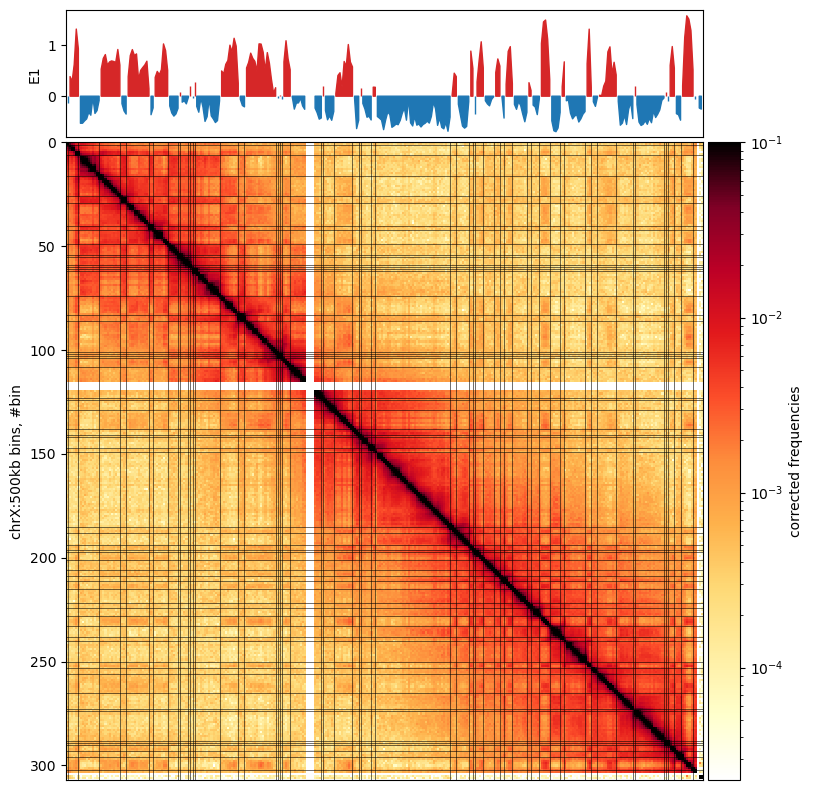
\includegraphics{index_files/figure-latex/..-..-notebooks-03_compartments-fig-matrix_e1_500kb-output-1.png}

}

\caption{\label{fig-matrix_e1_500kb}chrX interaction matrix with E1
eigenvector values in 500kb resolution. The sign change of the E1 is
overlayed as thin black lines, making it more easily interpretable. We
should qualitatively determine how well the E1 values capture the
\emph{plaid} pattern in the matrix.}

\end{figure}%

Here we see that Figure~\ref{fig-matrix_e1_500kb}\ldots{}

\section{Results}\label{results}

Here are the glorious results

\section{Discussion}\label{discussion}

Here is the discussion


\renewcommand\refname{Bibliography}
  \bibliography{sub-references.bib}



\end{document}
